\section{An initial overview of of the course}
\title[Initial overview]{Power Electronics Devices and Components}
 
\begin{frame}[plain]
    \titlepage
\end{frame}
%%%%%%%%%%%%%%%%%%%%%%%%%%%%%%%%%%%%%%%%%%%%%%%%%%%%%%%%%%%%%
%% Overview of the course %%
%%%%%%%%%%%%%%%%%%%%%%%%%%%%%%%%%%%%%%%%%%%%%%%%%%%%%%%%%%%%%
\begin{frame}
	\frametitle{Course Overview}
The course will be in 6 modules.
		\begin{itemize}
		  \item Module I: Introduction to Automation Technologies.
		  \item Module II: Sensor Technologies.
		  \item Module III: Signal Conditioning.
		  \item Module IV: Processors in Automation Systems.
		  \item Module V: Controllers and Communication.
%		  \item Module VI: Industrial communication systems.
		  \item Module VI: Actuators and Motion Systems.
		  \item Module VII: Testing and Validation.
		  \item Module VIII: Industrial Case Studies.
		\end{itemize}
\textbf{Pattern of class}: \\ Day: Tuesday, every week \\ 
Time: 8 am to 10 am (theory) and 10 am to 12 am (tutorial) (ideally but it can change) \\
Holidays: 23 Dec 2025, 30 Dec 2025, and 6 Jan 2026. %As required classes will be rescheduled. 
\end{frame}

%%%%%%%%%%%%%%%%%%%%%%%%%%%%%%%%%%%%%%%%%%%%%%%%%%%%%%%%%%%%%
%% Teaching Support Team %%
%%%%%%%%%%%%%%%%%%%%%%%%%%%%%%%%%%%%%%%%%%%%%%%%%%%%%%%%%%%%%
\begin{frame}
	\frametitle{The teaching team}
	\vspace{-0.5cm}
	\begin{columns}[t]
\centering
		\column[T]{0.33\textwidth}
		\begin{figure}
			\centering
				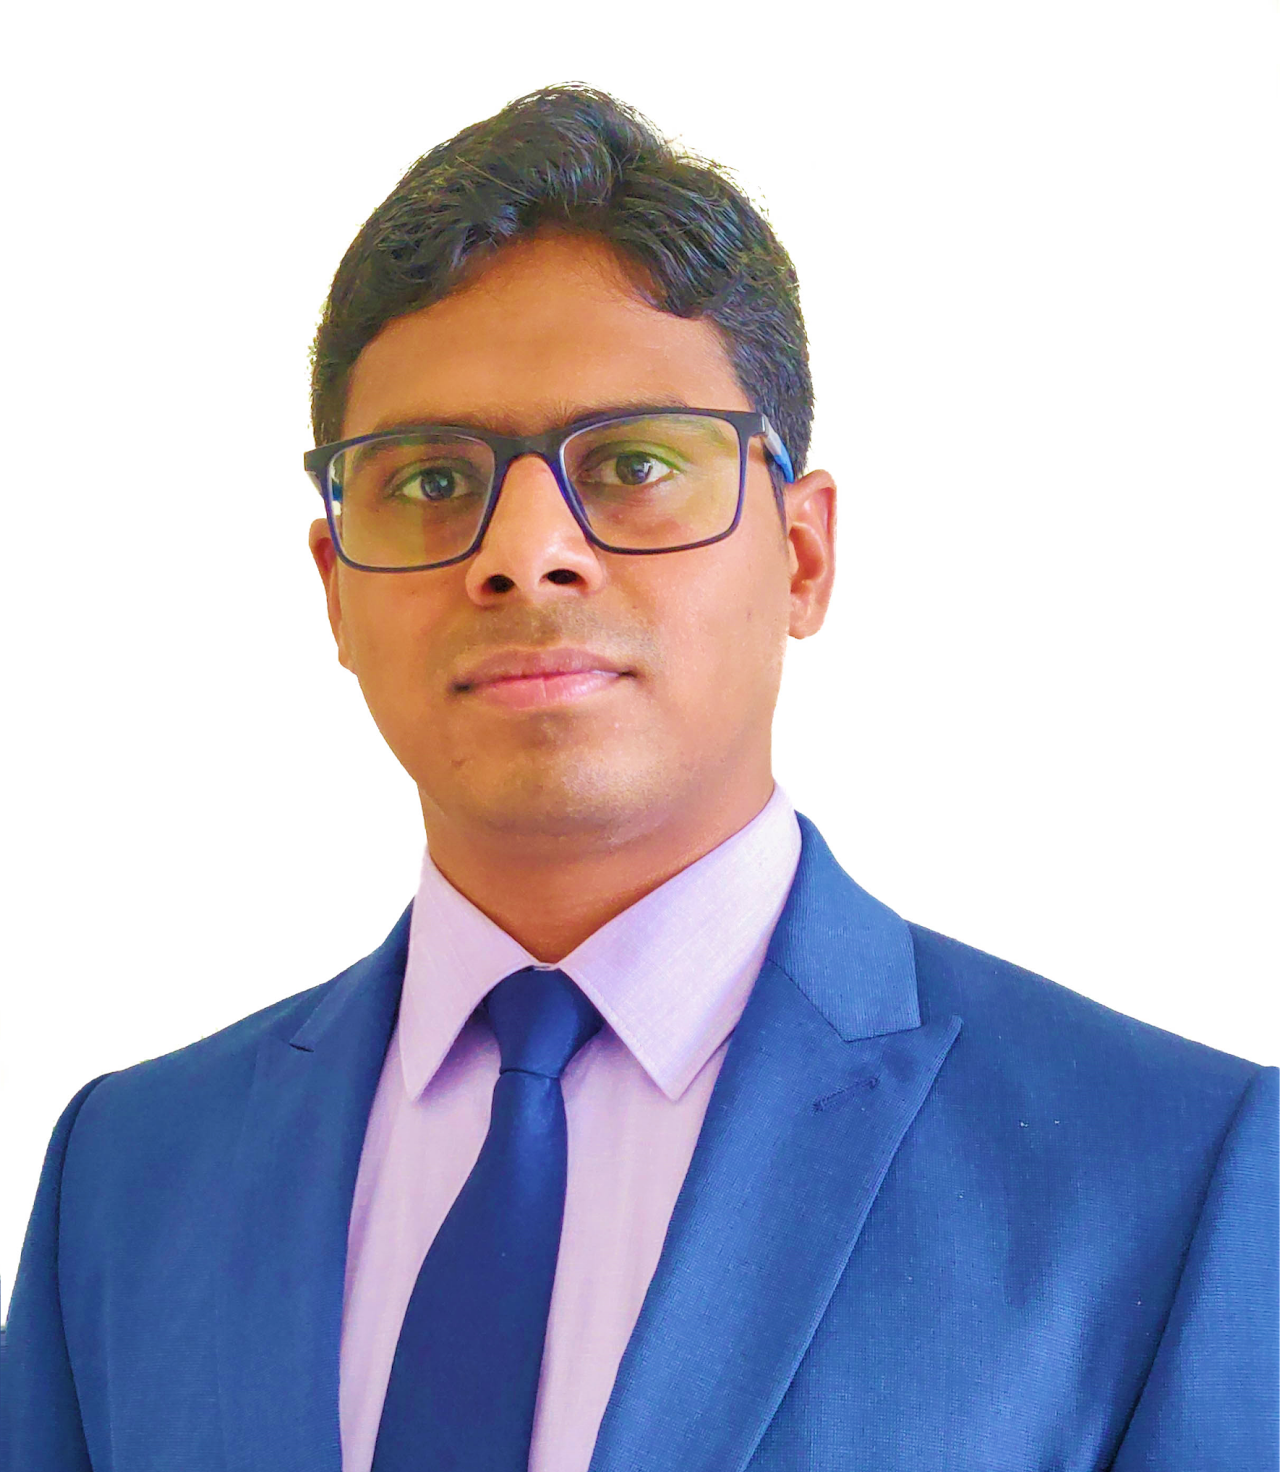
\includegraphics[height=2.5cm]{fig/lec01/Bikash.png}
				\caption*{Bikash Sah}
		\end{figure}
	
		\column[T]{0.33\textwidth}
		\begin{figure}
			\centering
				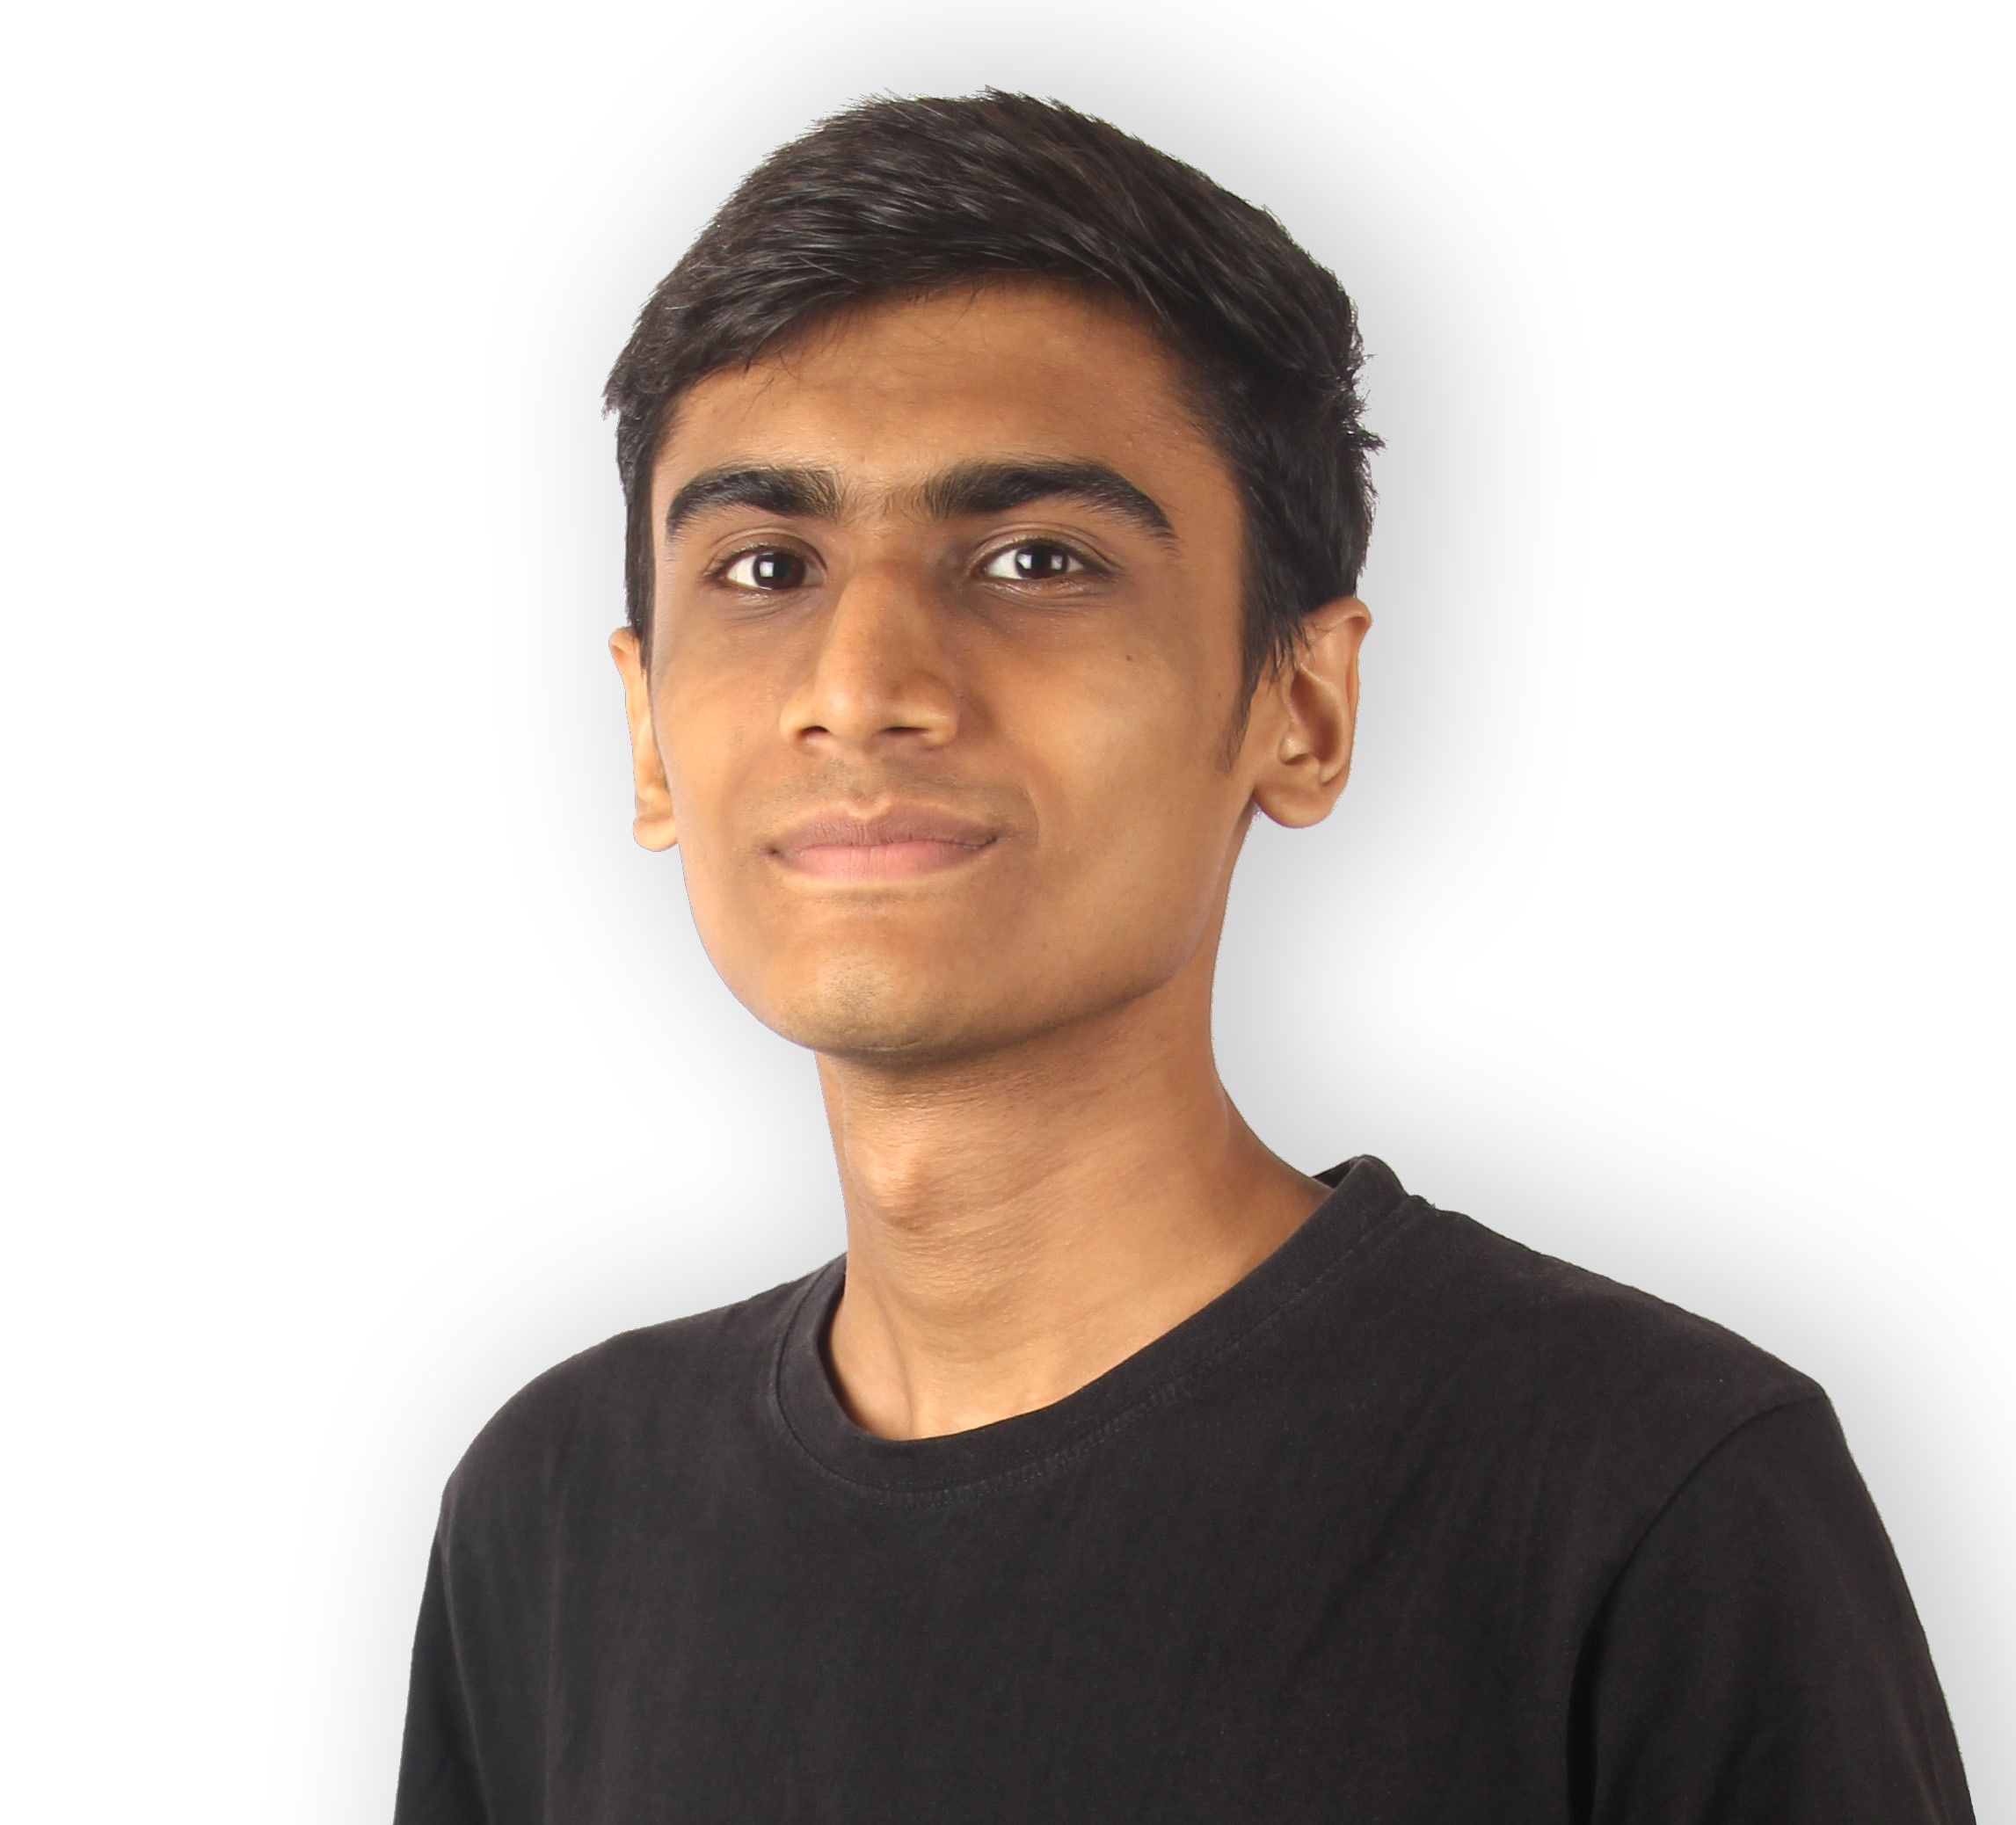
\includegraphics[height=2.5cm]{fig/lec01/Tatsat.jpg}
				\caption*{Tatsat Baldaniya}
		\end{figure}
		\column[T]{0.33\textwidth}
		\begin{figure}
			\centering
				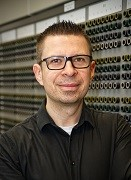
\includegraphics[height=2.5cm]{fig/lec01/pawel.jpg}
				\caption*{Pawel Malicki}
		\end{figure}		
	\end{columns}
	\vspace{-0.5cm}
	\begin{varblock}{Contact}
		\begin{itemize}
			\item Email: see \href{https://www.eti.uni-siegen.de/ias/}{chair's homepage}
			\item Offices: H-A building, 4th floor
			\item Individual appointments on request (remote or personally)
            \item Multiple relevant courses are offered by the Chair.  \href{https://www.eti.uni-siegen.de/ias/teaching/}{Check link!}
		\end{itemize}
	\end{varblock}
%** \small{Future follow-up courses are planned to be introduced in next semester- High Frequency Power Electronics, etc.}
	\end{frame}



%%%%%%%%%%%%%%%%%%%%%%%%%%%%%%%%%%%%%%%%%%%%%%%%%%%%%%%%%%%%%
%% Start %%
%%%%%%%%%%%%%%%%%%%%%%%%%%%%%%%%%%%%%%%%%%%%%%%%%%%%%%%%%%%%%
\begin{frame}
\center
\textbf{\huge{Module I: Introduction to Automation Technologies}}
\end{frame}

%%%%%%%%%%%%%%%%%%%%%%%%%%%%%%%%%%%%%%%%%%%%%%%%%%%%%%%%%%%%%
%% What is Electronics %%
%%%%%%%%%%%%%%%%%%%%%%%%%%%%%%%%%%%%%%%%%%%%%%%%%%%%%%%%%%%%%
% \begin{frame}
% 	\frametitle{What are "Electronic Devices"?}
% 	\begin{columns}
% 		\begin{column}{0.5\textwidth}
% 			\begin{varblock}{Electronic Devices}
% 				Electronic devices are hardware components which leverage the property of materials to control the flow of electrons or charge.
% 			\end{varblock} \vspace{-0.5cm}		
% 			\begin{itemize}
% 				\item<2-> Have a long history of development- started with the invention of vaccum tube or Thermionic valve in 1904 by J.A. Fleming.
% 				\item<3-> The first transistor was invented in 1947 by J.Bardeen, W.H. Brattain and W.S. Shockley in Bell Labs.
% 				\item<4-> The first integrated circuit was invented in 1958 by J. Kilby and R. Noyce -- On and it goes
% %				\item<5-> The first microprocessor was invented in 1971 by F. Faggin, T. Klein and H. Hoff in Intel.
% %				\item<6-> The first microcontroller was invented in 1971 by F. Faggin, T. Klein and H. Hoff in Intel.
% %				\item<7-> On and it goes- every day new devices are invented and developed.
% 			\end{itemize}
% 		\end{column}
% 		\begin{column}{0.5\textwidth}
% 			\begin{figure}
% 				\centering
% 				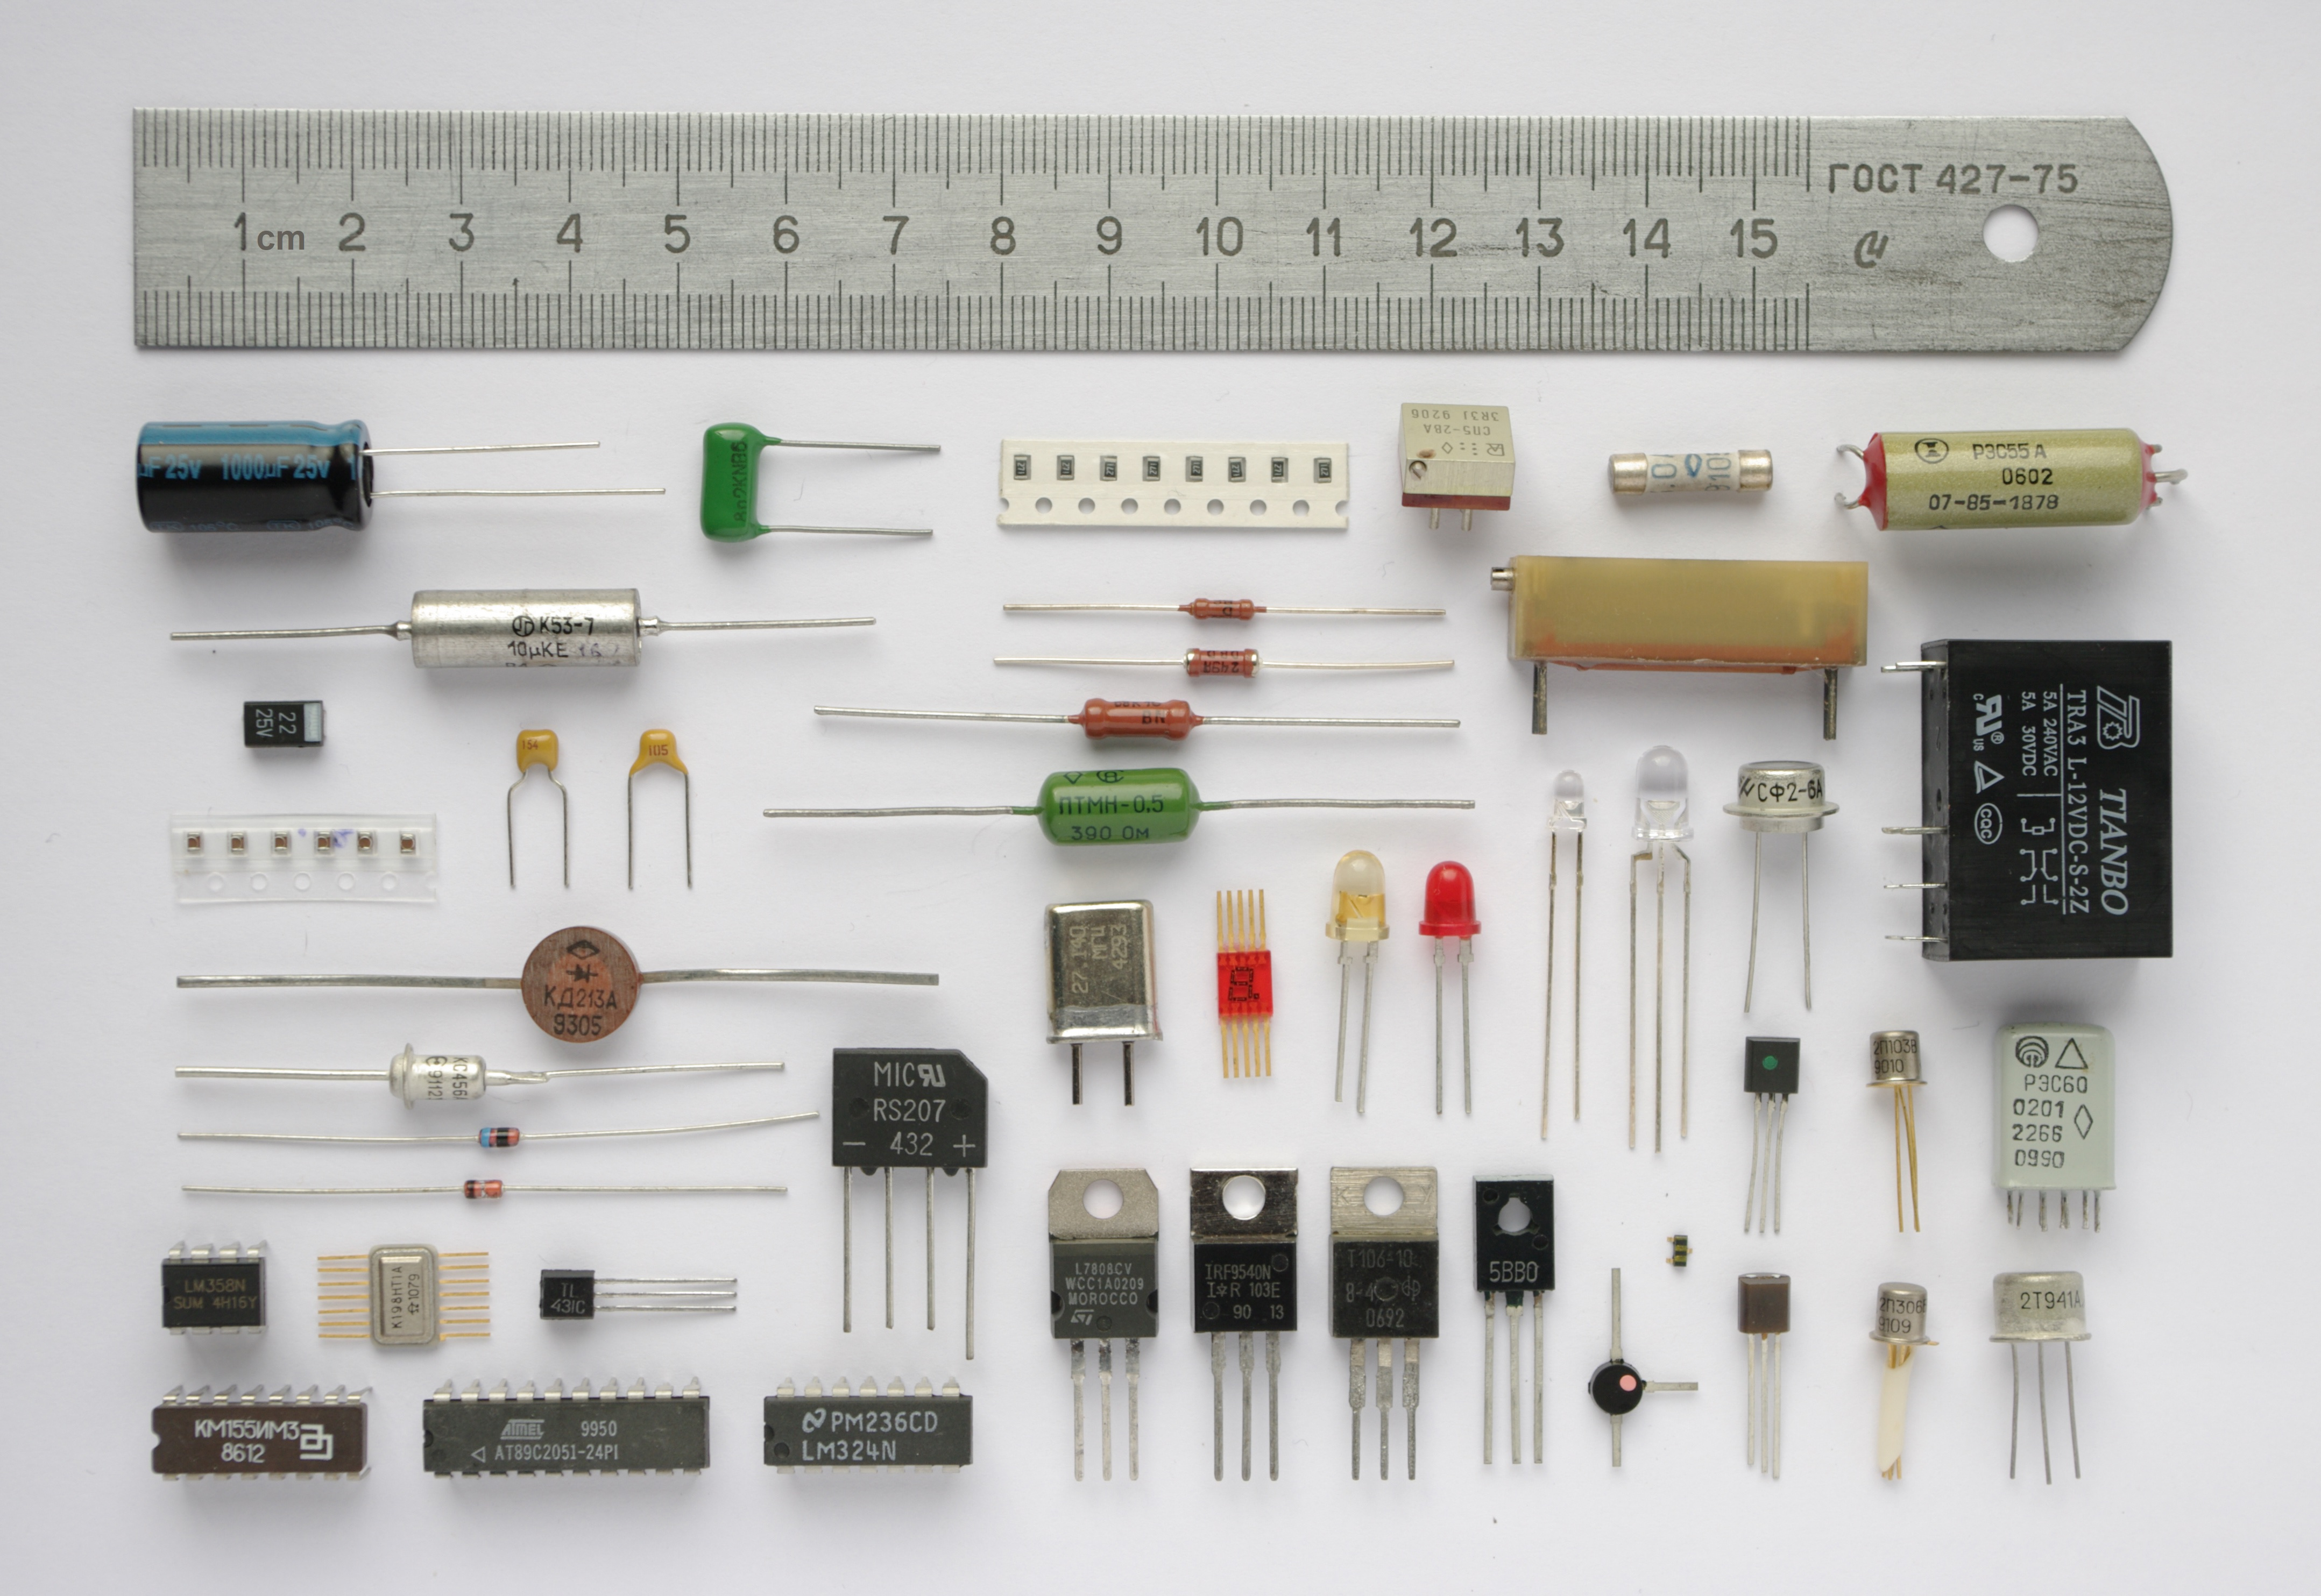
\includegraphics[scale= 0.05]{fig/lec01/Componentes.jpg}
% 				\caption{Example of electronic components (source: \href{https://commons.wikimedia.org/wiki/File:Componentes.JPG}{Wikimedia Commons}, Kae, public domain)}
% 			\end{figure}
% 		\end{column}
% 		\end{columns}
% \end{frame}



% --- Slide 1: What is Automation? ---
\begin{frame}{What is \textit{Automation}?}
\textbf{Working definition for this course}\\[2mm]
\emph{Automation is the purposeful application of mechanical, electrical, and computer technologies to reduce human involvement in task performance-without necessarily removing humans from the loop.}

Highly interdisciplinary, it encompasses: combine elements of sensor technology, actuator technology, control technology, communication technology, real-time software, and data science, among other things.

\vspace{2mm}
\textbf{Key nuances}
\begin{itemize}
  \item \textbf{Displace vs. replace:} automation often reallocates human effort to higher-value tasks rather than eliminating it.
  \item \textbf{Hardware and software co-design:} improvement may be purely software (e.g., CAD workflows) or mechatronic (robotic cells).
  \item \textbf{Beyond factories:} retail checkout, medical devices, energy systems, mobility-all are automation domains.
\end{itemize}

%\vspace{2mm}
\end{frame}

\begin{frame}{Examples of Automation}
%\textbf{Illustrative examples}
	\begin{columns}
		\begin{column}{0.25\textwidth}
			\begin{itemize}
  				\item \emph{Self-checkout:} barcode + payment automation reduces repetitive cashier tasks while keeping supervision.
			\end{itemize}
		\end{column}
		\begin{column}{0.75\textwidth}
				\begin{figure}
				\centering
				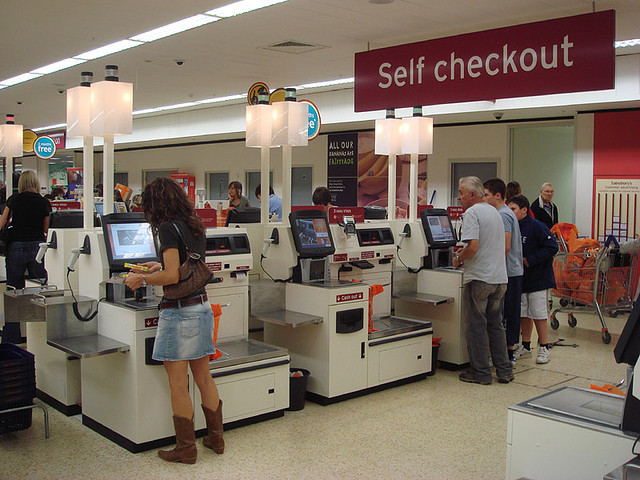
\includegraphics[width=0.7\linewidth]{fig/lec01/Self_checkout.jpg}
				\caption*{Self checkout machines (Source: from \href{https://commons.wikimedia.org/wiki/File:Self_checkout_using_NCR_Fastlane_machines.jpg}{Self checkout using NCR Fastlane machines}, \href{https://creativecommons.org/licenses/by/2.0/deed.en}{CC BY 2.0})}
			\end{figure}
		\end{column}
\end{columns}
\end{frame}

\begin{frame}{Examples of Automation}
%\textbf{Illustrative examples}
	\begin{columns}
		\begin{column}{0.25\textwidth}
			\begin{itemize}
				\item \emph{Computer Aided Design (CAD) evolution:} from manual drafting to 3D solid modeling, numerical control code, and auto-documentation.
			\end{itemize}
		\end{column}
		\begin{column}{0.75\textwidth}
				\begin{figure}
				\centering
				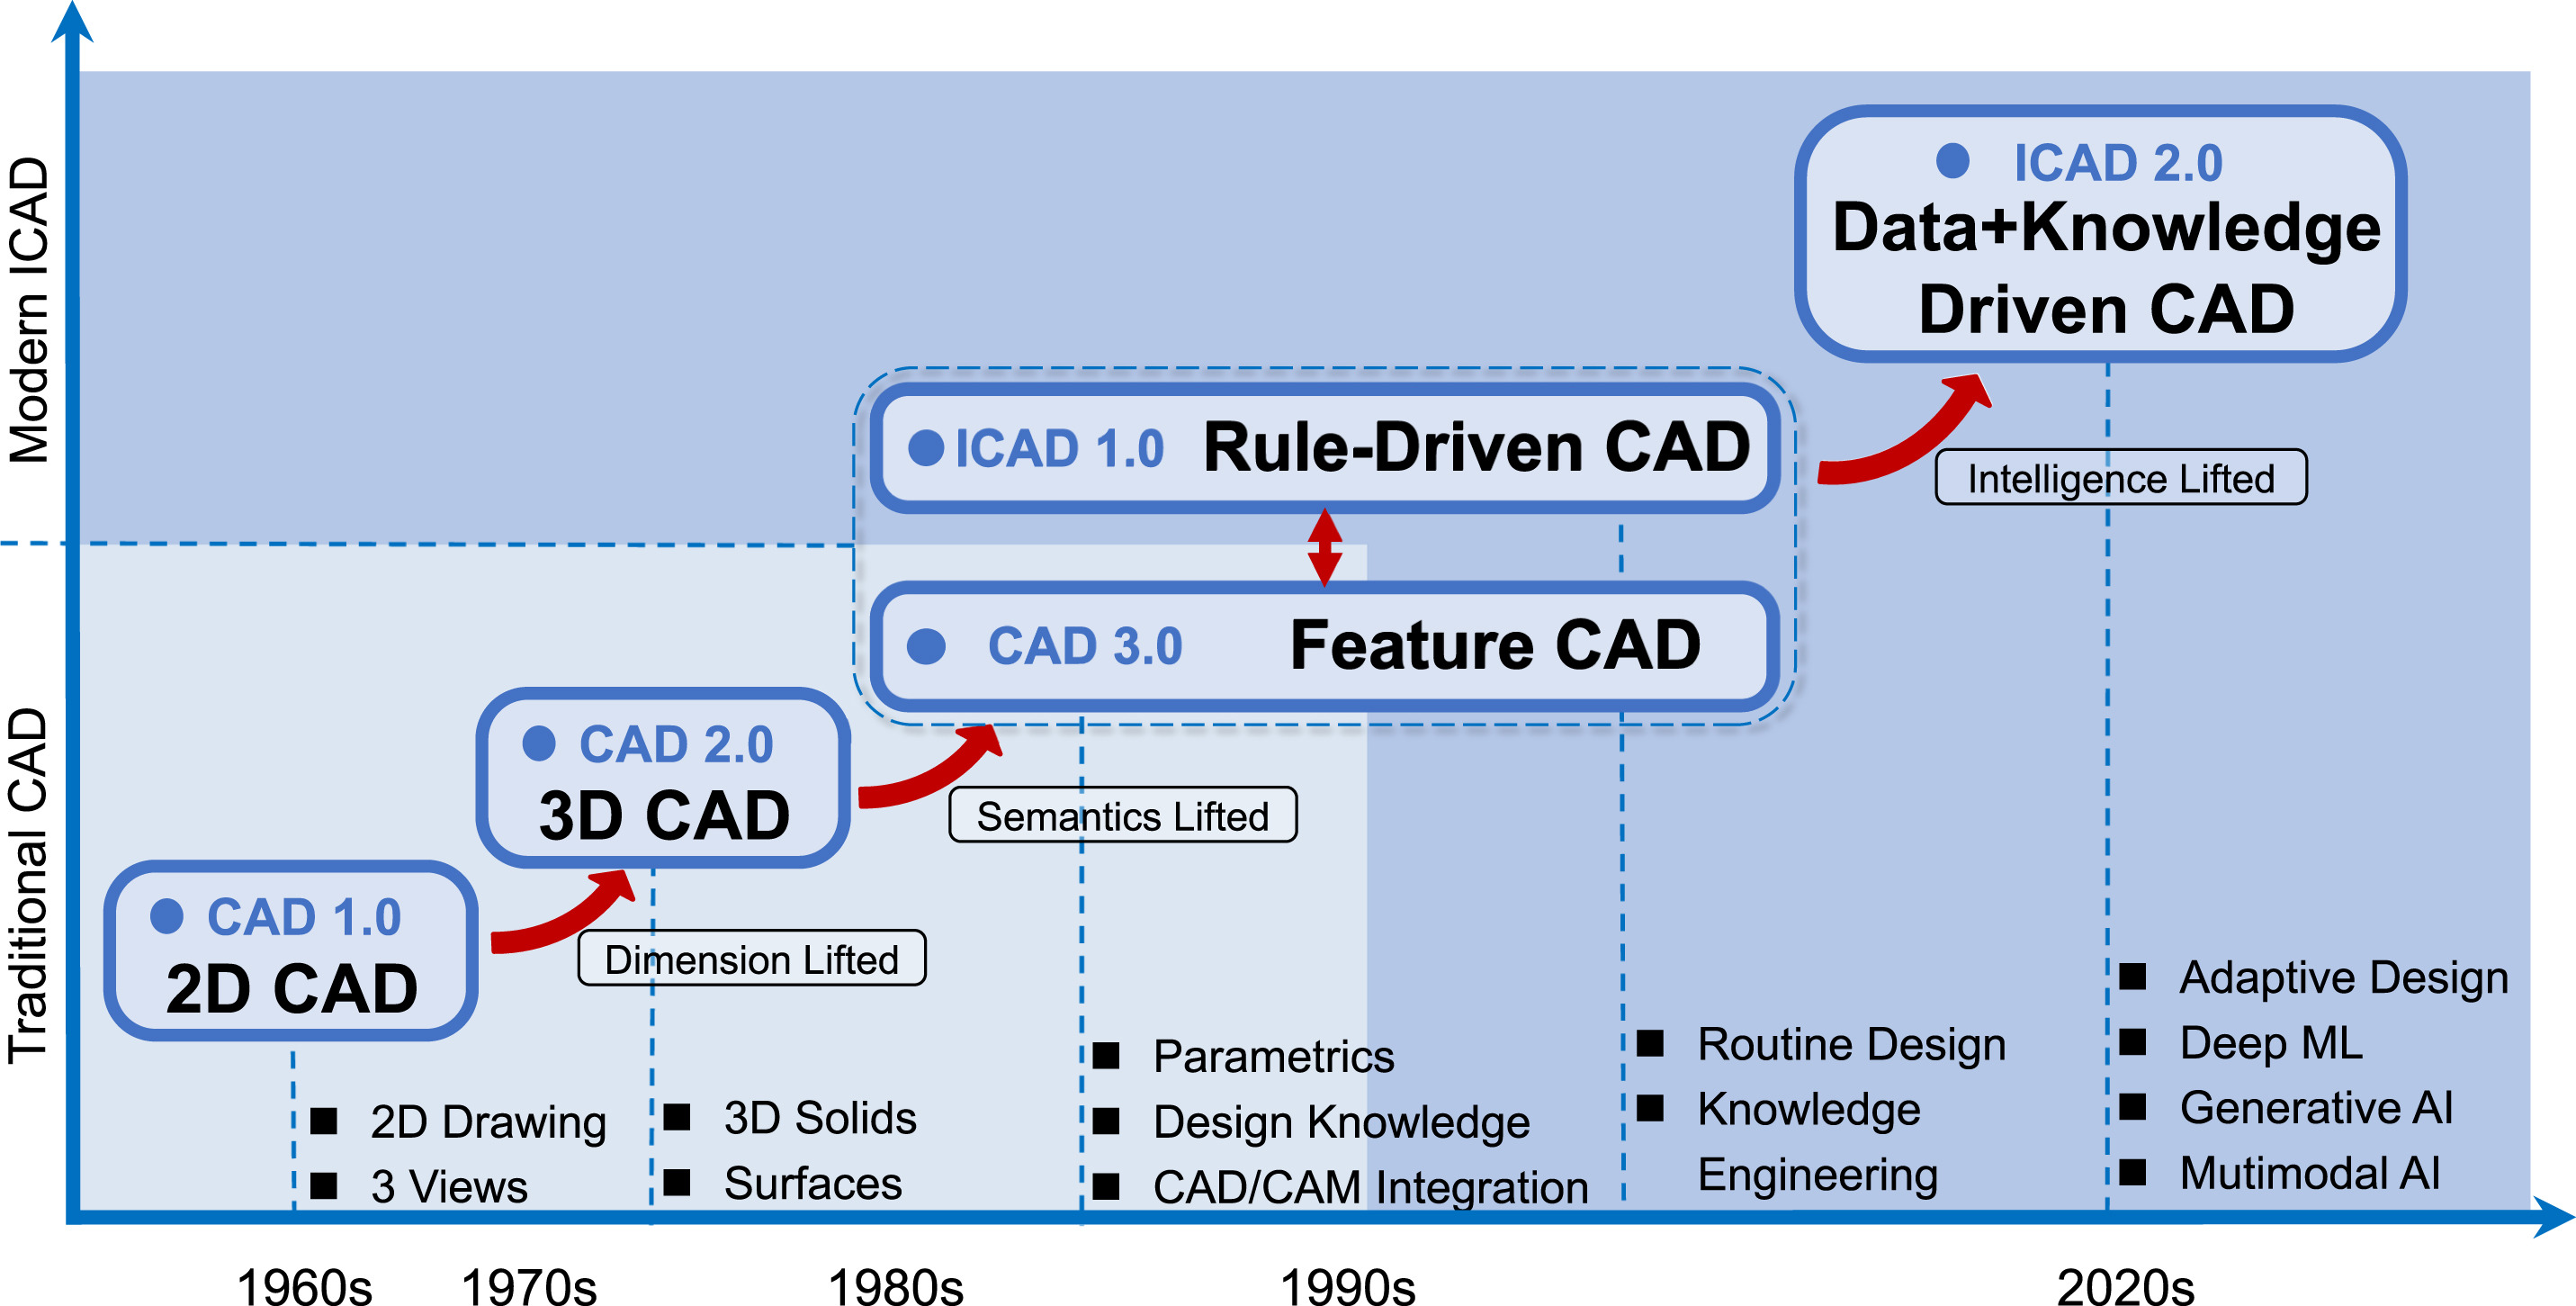
\includegraphics[width=0.8\linewidth]{fig/lec01/CAD_development.jpg}
				\caption*{Historical development of CAD (Source: Zou, Qiang, Yingcai Wu, Zhenyu Liu, Weiwei Xu, and Shuming Gao. "Intelligent CAD 2.0." Visual Informatics 8, no. 4 (2024): 1-12.)}
			\end{figure}
		\end{column}
\end{columns}
\end{frame}




% --- Slide 2: Why Now? Value & Impact ---
\begin{frame}{Why Now? Value, Impact, and Trends}
\textbf{What automation accomplishes today}
\begin{itemize}
  \item Enables \textbf{flexible value networks}: rapid changeovers, mass customization, and supply-chain visibility.
  \item Integrates \textbf{heterogeneous technologies} across disciplines; links physical assets to \textbf{digital representations}.
  \item Improves \textbf{quality, safety, and energy efficiency}; turns data into decisions.
\end{itemize}

\textbf{Where it is going}
\begin{itemize}
  \item From real-time control of single machines to \textbf{orchestration} of whole cells/lines and ecosystems.
  \item \textbf{Autonomous capabilities}: perception, context understanding, and bounded autonomy with human oversight.
  \item \textbf{Sustainability and circularity}: traceability, footprint accounting, and lifecycle optimization.
\end{itemize}
\end{frame}


\begin{frame}{Why Now? Value, Impact, and Trends}
	\begin{columns}
		\begin{column}{0.25\textwidth}
			\textbf{Practical life example}\\
				Battery cycler cell: recipe engine (e.g., CC-CV-rest), interlocks, data historian, remote diagnostics, and energy-aware scheduling.
		\end{column}
		\begin{column}{0.75\textwidth}
				\begin{figure}
				\centering
				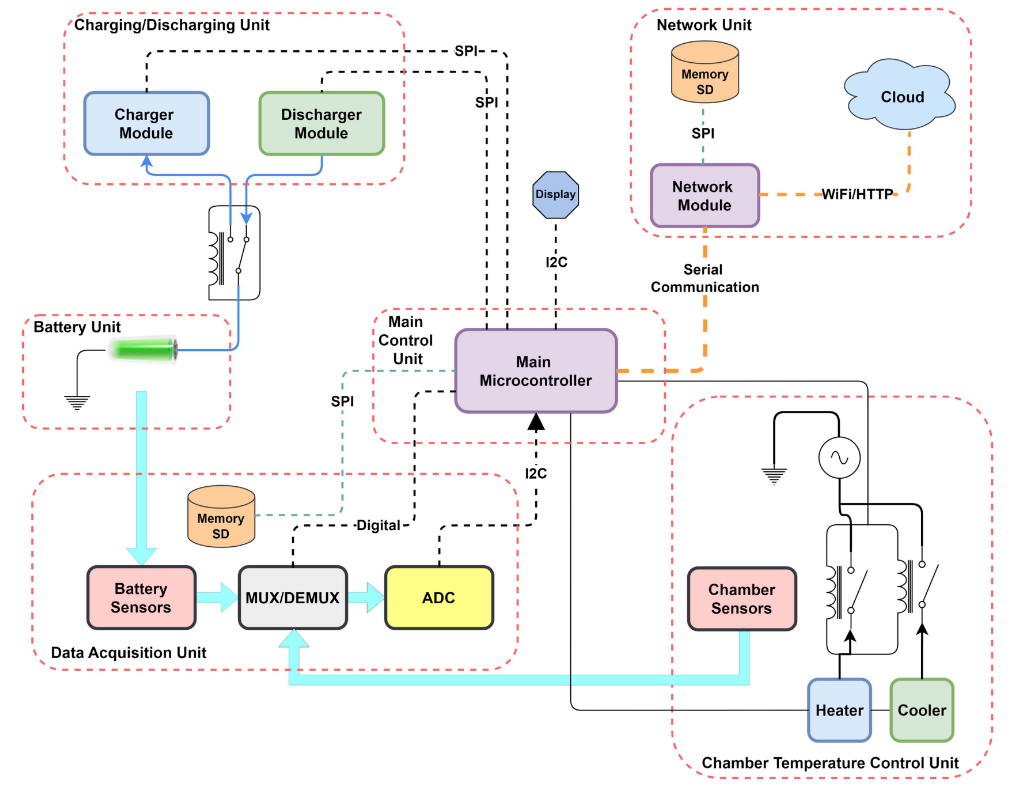
\includegraphics[width=0.7\linewidth]{fig/lec01/cell_test_automation.png}
				\caption*{Automated cell test set-up (Source: \href{https://doi.org/10.1109/TIA.2025.3561705}{Mulpuri et. al.,IEEE Trans. on Industry Appl., vol. 61-5})}
			\end{figure}
		\end{column}
\end{columns}
\end{frame}


\begin{frame}{Nature and Scope of Automation}
\textbf{Automation can occur anywhere humans perform structured tasks.}
\begin{itemize}
  \item Includes entertainment (remote controls), offices (data entry), transportation, and healthcare.
  \item Combines mechanical, electrical, and computer elements-modern systems are hybrid and interlinked.
  \item Machines themselves can contain smaller automated subsystems, leading to hierarchical automation.
\end{itemize}

\vspace{3mm}
\textbf{Essence:}  
Automation evolves continually, driven by technology that reduces human effort, improves precision, and enhances reliability across diverse applications.
\end{frame}

\begin{frame}{Automation Technology Today and Tomorrow}
\textbf{Current accomplishments :} as per the Society for Measurement and Automation Technology within the Association of German Engineers (VDI/VDE) outlook\footnotemark:
\begin{itemize}
  \item Enables \textbf{flexible value networks} and digital connectivity.
  \item Makes technology more accessible and user-friendly.
  \item Integrates mechanical, electrical, and information technologies.
  \item Connects \textbf{real-world physical elements} with their \textbf{digital representations}.
\end{itemize}

\vspace{3mm}
\textbf{Emerging directions}
\begin{itemize}
  \item Intelligent, networked products capable of autonomous action.
  \item Sustainability and circular economy supported by digital transparency.
  \item Need for clear standards, security, and qualified human oversight.
\end{itemize}
\footnotetext[1]{Adamczyk et. al., Automation 2025—Hypotheses and fields of action. (in German) VDI/VDE Society for Measurement and Control, 2015}
\end{frame}

\begin{frame}{Self-Perception of Automation Technology}
\textbf{A multidisciplinary field:}
\begin{itemize}
  \item Integrates \textbf{mechanical, electrical, computer, and information engineering}.
  \item Engineers act as \textbf{system integrators}-coordinating diverse components into a coherent whole.
\end{itemize}

\vspace{3mm}
\textbf{Historical evolution:}
\begin{itemize}
  \item From mechanical aids to networked, software-defined systems.
  \item Increased productivity and flexibility through information technology.
\end{itemize}

\vspace{3mm}
\textbf{Future perspective:}
\begin{itemize}
  \item Toward \textbf{autonomous systems} that perceive, decide, and act.
  \item Humans remain central-for supervision, creativity, and ethical responsibility.
\end{itemize}
\end{frame}


\begin{frame}
	\frametitle{Examples of automation technologies (2)}
	% Set up a 2x2 grid of figures
	\begin{figure}
		\centering
		\begin{subfigure}[b]{0.49\textwidth}
			\centering
			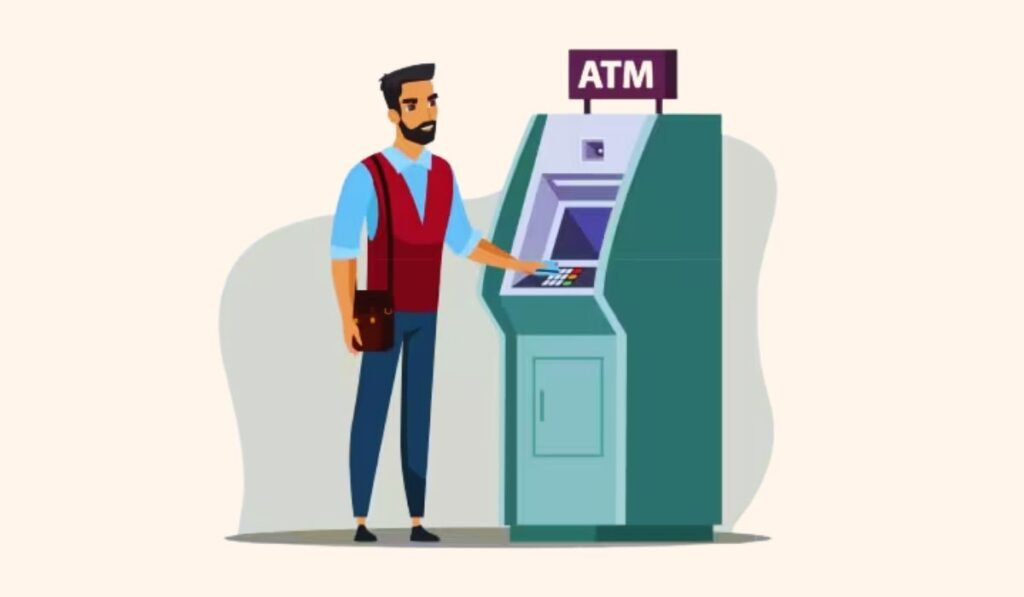
\includegraphics[width=0.5\textwidth]{fig/lec01/ATM}
			\caption{ATM (source: \href{https://www.paymeindia.in/blog/wp-content/uploads/2025/02/what-is-an-atm-1024x597.jpg}{PayMe}, public domain)}
		\end{subfigure}
		\hfill
		\begin{subfigure}[b]{0.49\textwidth}
			\centering
			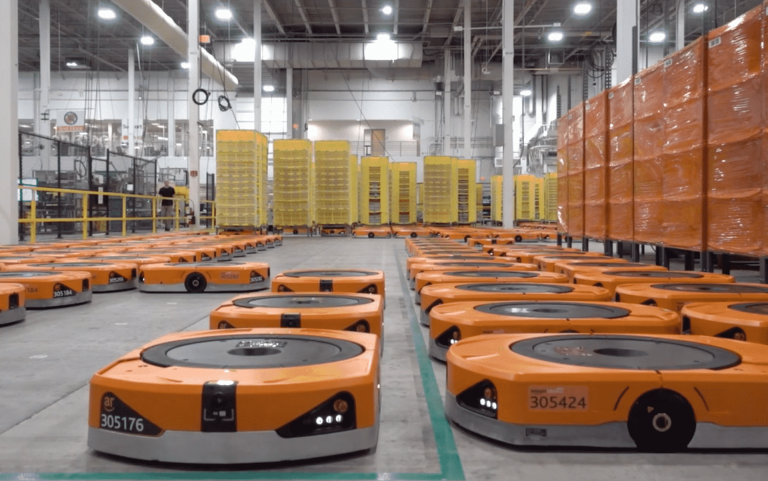
\includegraphics[width=0.5\textwidth]{fig/lec01/Amazon.png}
			\caption{Amazon Robotic Fulfillment Center (source: \href{https://www.waredock.com/wp-content/uploads/2019/08/Screenshot-2019-08-01-at-22.50.57-768x481.png}{Waredock eCommerce Fulfilment Network}, public domain)}
		\end{subfigure}
		\\
		\begin{subfigure}[b]{0.49\textwidth}
			\centering
			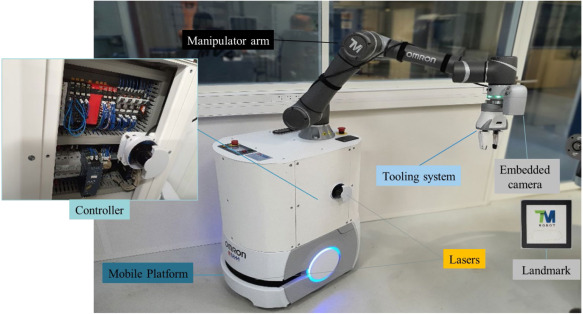
\includegraphics[width=0.5\textwidth]{fig/lec01/PLC.jpg}
			\caption{PLC Controller used in Mobile 
Robots (source: \href{https://doi.org/10.1016/j.robot.2023.104526}{Ghodsian et. al.})}
		\end{subfigure}
		\hfill
		\begin{subfigure}[b]{0.49\textwidth}
			\centering
			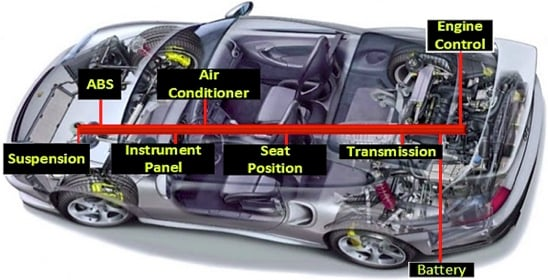
\includegraphics[width=0.5\textwidth]{fig/lec01/CAN.jpg}
			\caption{CAN Bus is used for ECU 
communication in cars (source: \href{https://www.allaboutcircuits.com/uploads/articles/CAN.jpg}{Wikimedia Commons}, Stephen St. Michael, \href{https://www.allaboutcircuits.com/technical-articles/introduction-to-can-controller-area-network/}{ Introduction to CAN (Controller Area Network) })}
		\end{subfigure}
		\vspace{-0.5cm}
		\caption*{Examples of automation technologies in various domains} 
        \label{fig:examples_machine_drives_02}
	\end{figure}
\end{frame}

\begin{frame}
	\frametitle{Examples of automation technologies (1)}
	\begin{figure}
		\centering
		\begin{subfigure}[b]{0.49\textwidth}
			\centering
			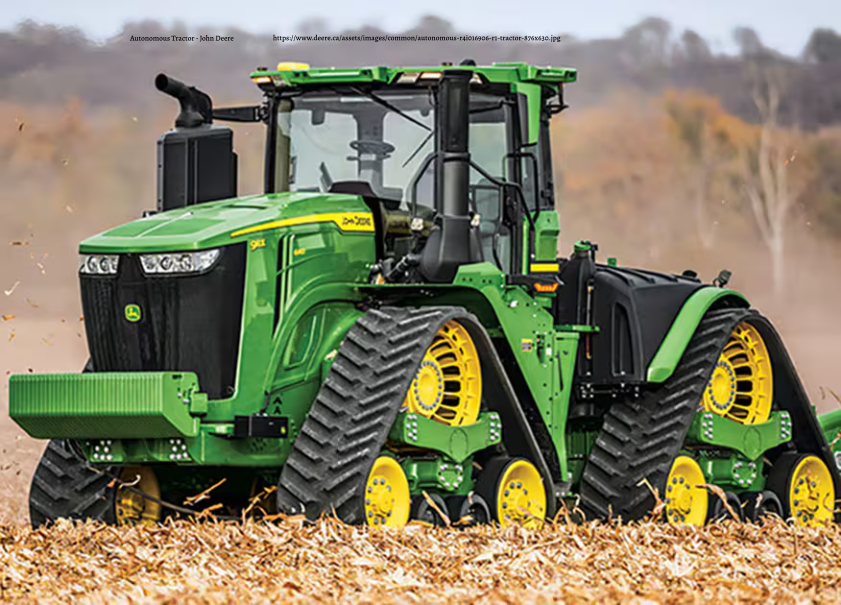
\includegraphics[width=0.5\textwidth]{fig/lec01/Tractor.png}
			\caption{John Deere's autonomous tractor (source: \href{https://www.deere.ca/assets/images/common/autonomous-r4i016906-r1-tractor-876x630.jpg}{Why Do I Need Autonomy?},  Deere \& Company, public domain)}
		\end{subfigure}
		\hfill
		\begin{subfigure}[b]{0.49\textwidth}
			\centering
			\includegraphics[width=0.5\textwidth]{fig/lec01/A340_FCU.jpg}
			\caption{The modern flight control unit of an Airbus A340 (source: \href{https://pxhere.com/en/photo/954757}{pxhere.com}, K A Salom, \href{https://creativecommons.org/licenses/by/2.0}{CC BY 2.0})}
		\end{subfigure}
		\\ 
		\vspace{-0.25cm}
		\begin{subfigure}[b]{0.49\textwidth}
			\centering
			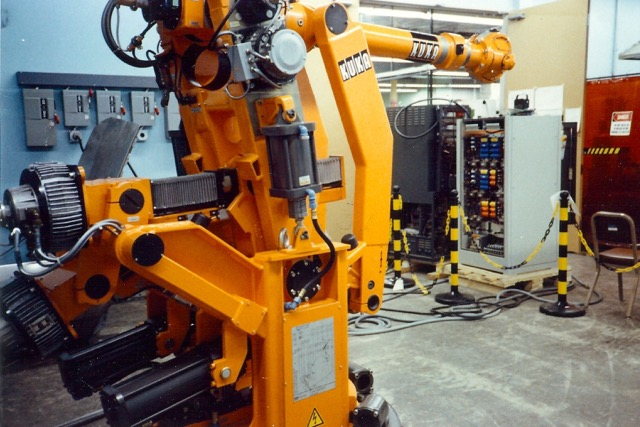
\includegraphics[width=0.5\textwidth]{fig/lec01/Automatix_KukaRobot.jpg}
			\caption{Factory robots (source: \href{https://commons.wikimedia.org/wiki/File:Automatix_KukaRobot483.agr.jpg}{Wikimedia Commons}, A.~Reinhold, \href{https://creativecommons.org/licenses/by-sa/4.0/deed.en}{CC BY-SA 4.0})}
		\end{subfigure}
		\hfill
		\begin{subfigure}[b]{0.49\textwidth}
			\centering
			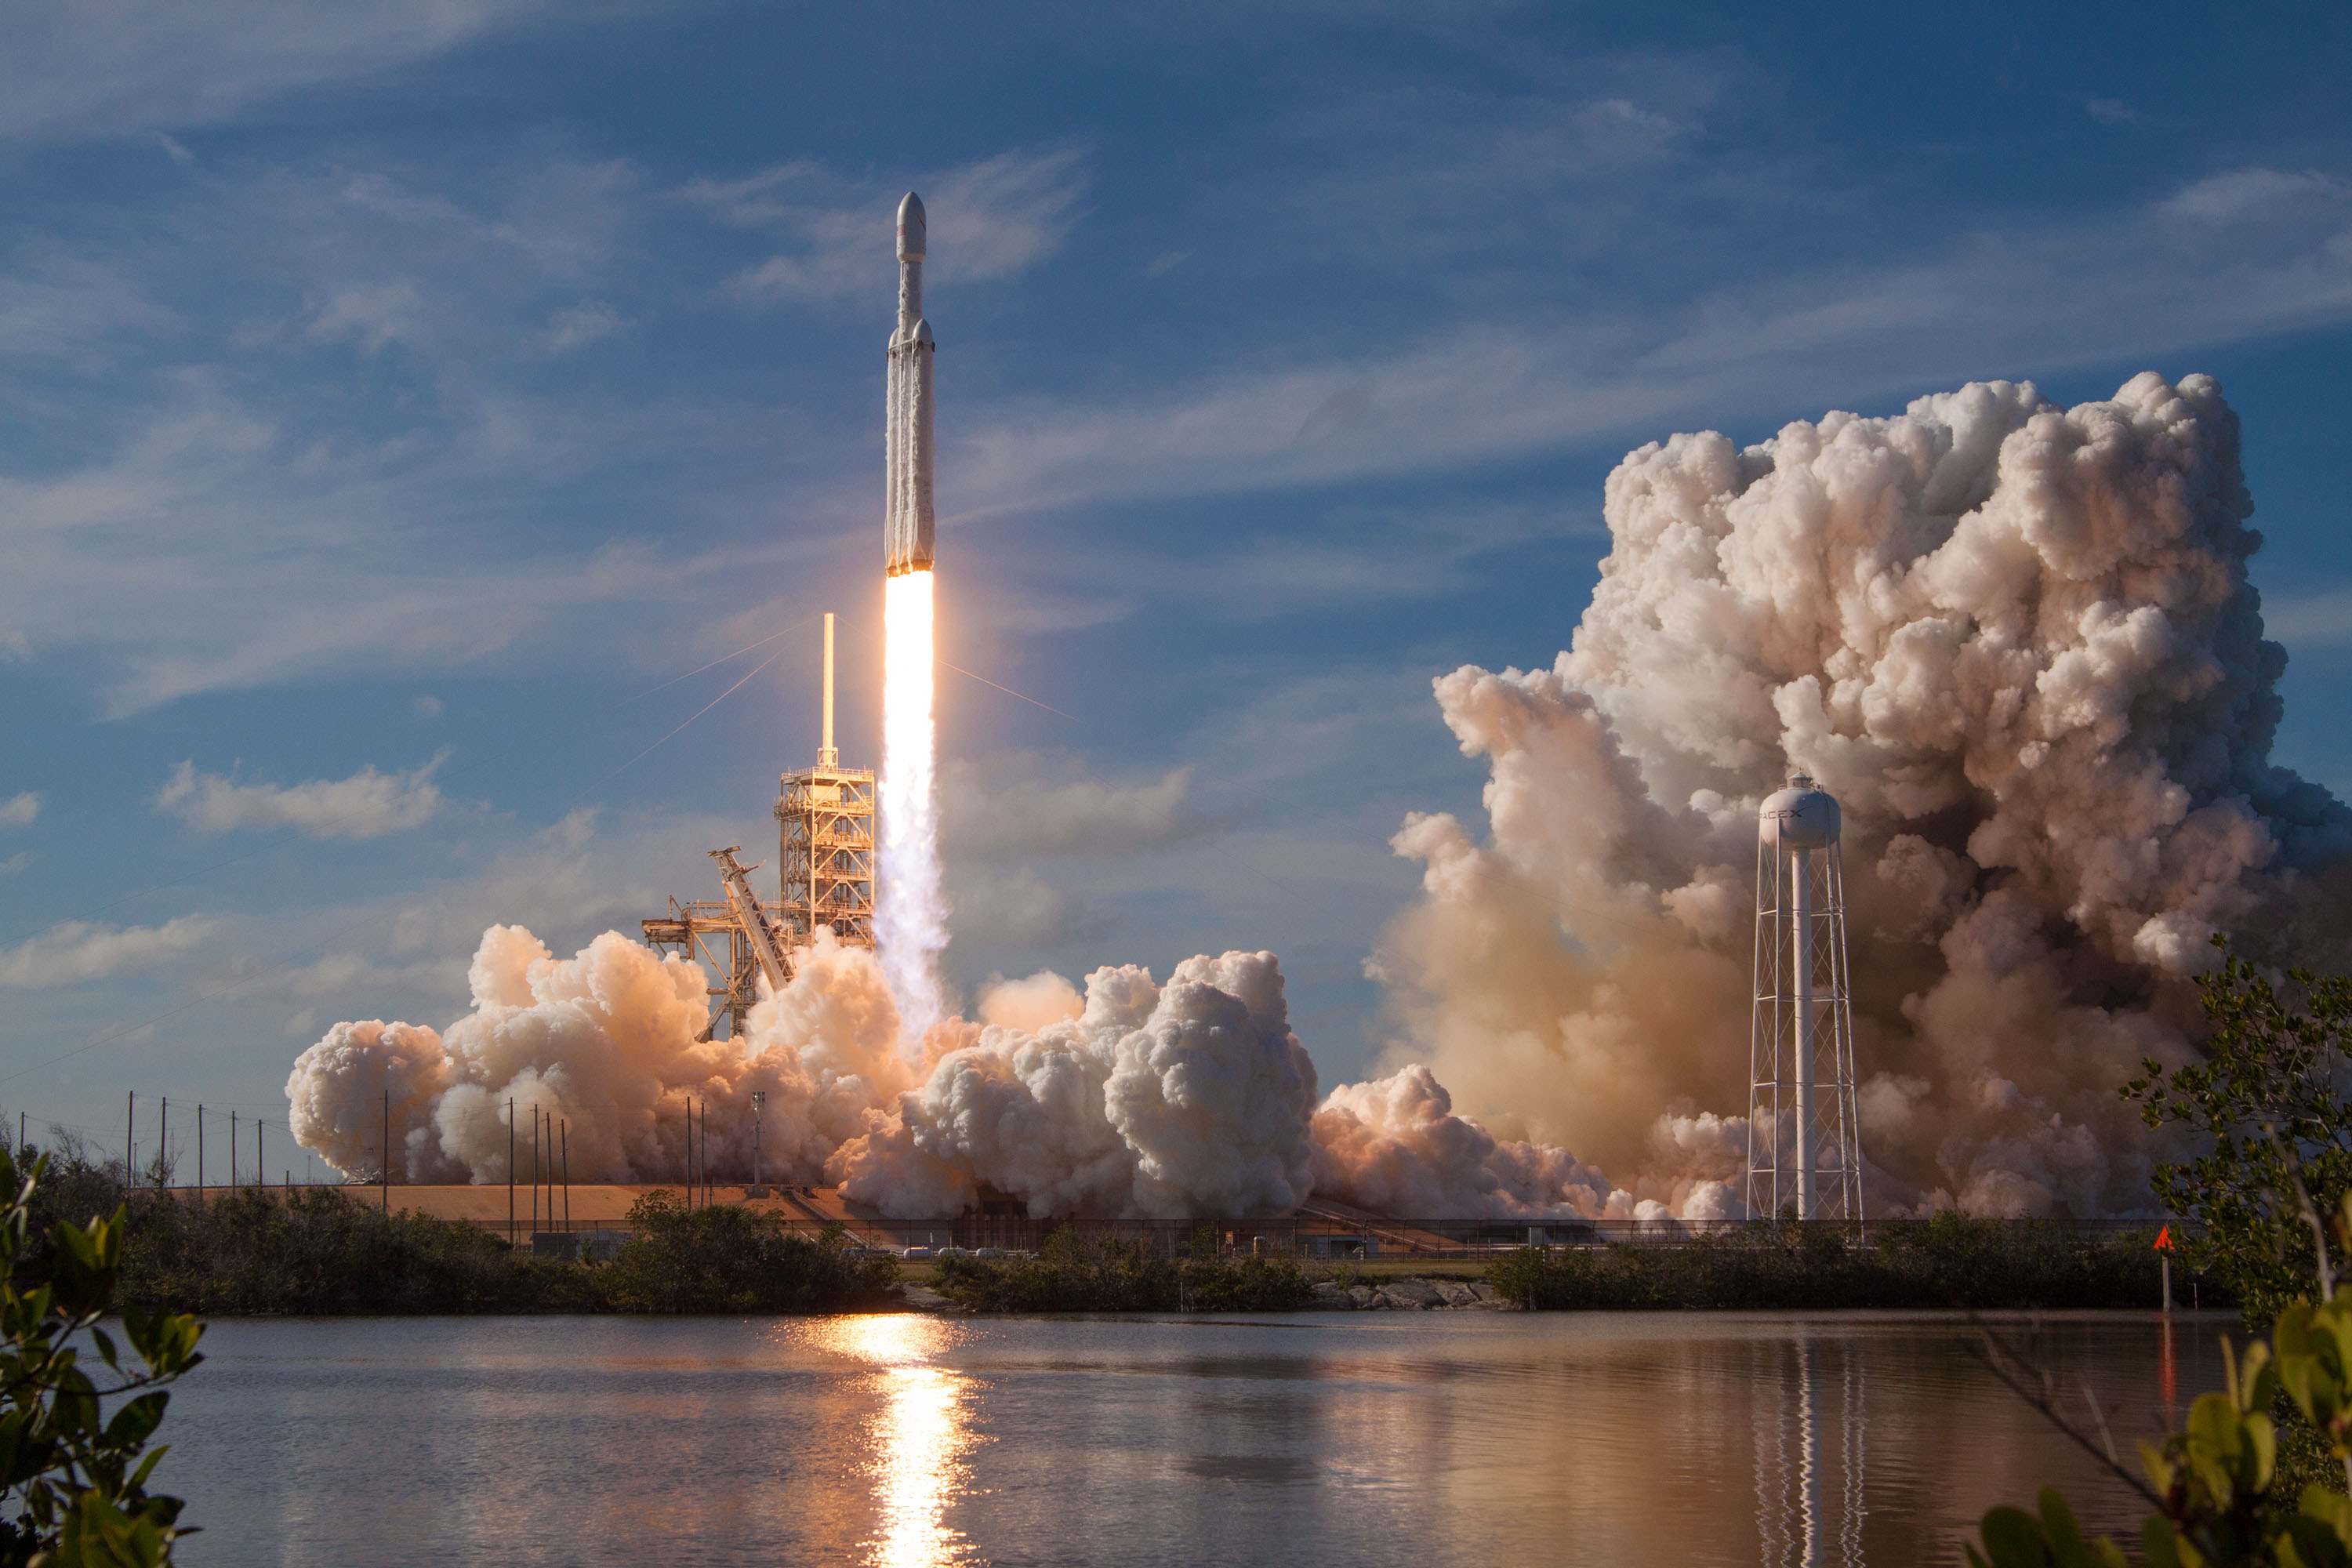
\includegraphics[width=0.5\textwidth]{fig/lec01/Falcon_Heavy_Demo_Mission_(40126461851).jpg}
			\caption{SpaceX Automated Guidance System (source: \href{https://commons.wikimedia.org/wiki/File:Falcon_Heavy_Demo_Mission_(40126461851).jpg}{Wikimedia Commons},  \href{https://creativecommons.org/public-domain/cc0/}{CC0})}
		\end{subfigure}
		\vspace{-0.5cm}
		\caption*{Examples of automation technologies in various domains} 
        \label{fig:examples_machine_drives_01}
	\end{figure}
\end{frame}

\begin{frame}{Automation - example case of manufacturing systems}
\textbf{Automation in manufacturing} can appear in:
\begin{itemize}
  \item \textbf{Manufacturing support systems} - e.g., Computer aided design (CAD), computer aided manufacturing (CAM), computer-integrated manufacturing (CIM) $^*$, and material requirement planning (MRP).
  \item \textbf{Manufacturing systems} - the actual production and material-handling equipment.
\end{itemize}

$^*$\textbf{Computer-integrated manufacturing (CIM)} links both levels by connecting support systems directly with factory automation for a fully integrated enterprise.

\vspace{3mm}
\textbf{Focus of this section:}\\
Automation that directly reduces the level of human participation in manufacturing processes.

\vspace{3mm}
\textbf{Three principal types of automation:}
\begin{enumerate}
  \item Fixed automation
  \item Programmable automation
  \item Flexible automation
\end{enumerate}
\end{frame}

%------------------------------------------------
\begin{frame}{Fixed Automation}
\textbf{Definition:}  
Equipment designed to perform a specific sequence of operations for one product or family of products.

\vspace{2mm}
\textbf{Key characteristics}
\begin{itemize}
  \item High \textbf{production rates}, low to high product complexity.
  \item Very limited product variety; reconfiguration requires major setup time.
  \item High initial cost but low unit cost at large volumes.
  \item Typical of flow-line and assembly systems.
\end{itemize}

\vspace{3mm}
\textbf{Examples:}
\begin{itemize}
  \item Transfer lines for engine blocks.
  \item Automated bottling or packaging lines.
  \item Semiconductor assembly lines.
\end{itemize}

\vspace{3mm}
\textbf{Technology note:}  
Modern fixed systems may embed PLCs or computer control for limited adaptability, but mechanical configuration remains largely fixed.
\end{frame}

%------------------------------------------------
\begin{frame}{Programmable Automation}
\textbf{Definition:}  
Automation that allows the operating sequence or equipment configuration to be changed through program modification.

\vspace{2mm}
\textbf{Key characteristics}
\begin{itemize}
  \item Handles \textbf{moderate product variety} and \textbf{medium production volumes}.
  \item Reprogramming enables new tasks, but setup/changeover time can be long.
  \item Combines mechanical flexibility with electronic control.
  \item Core element of almost all modern automated systems.
\end{itemize}

\vspace{3mm}
\textbf{Enabling technologies:}
\begin{itemize}
  \item \textbf{CNC (Computer Numerical Control)} - programmable motion and tool paths.
  \item \textbf{Robotic technology} - reprogrammable manipulators for various tasks.
  \item \textbf{PLC (Programmable Logic Control)} - discrete logic sequencing and interlocks.
\end{itemize}

\vspace{3mm}
\textbf{Used in:} Machining, welding, assembly, and process industries.
\end{frame}

%------------------------------------------------
\begin{frame}{Flexible Automation}
\textbf{Definition:}  
An extension of programmable automation with \textbf{no lost time for changeover} between products.

\vspace{2mm}
\textbf{Key characteristics}
\begin{itemize}
  \item Capable of producing different parts in any order with little or no manual intervention.
  \item Combines features of fixed and programmable automation.
  \item Uses integrated computer control, sensors, and communication networks to recognize and adjust to part variations automatically.
  \item Supports \textbf{high product variety} and \textbf{moderate to high production rates}.
\end{itemize}

\vspace{3mm}
\textbf{Examples:}
\begin{itemize}
  \item Flexible manufacturing systems (FMS).
  \item CNC machining cells with automatic tool changers and pallet systems.
  \item Robotized assembly lines with vision feedback.
\end{itemize}
\end{frame}

%------------------------------------------------
\begin{frame}{Comparison of Automation Types}
\centering
\resizebox{\linewidth}{!}{
\begin{tabular}{lcccc}
\toprule
\textbf{Type} & \textbf{Product Complexity} & \textbf{Product Variety} & \textbf{Production Volume} & \textbf{System Type}\\
\midrule
Fixed        & Low–High & None      & High       & Flow-line\\
Programmable & High     & Hard      & Moderate   & All types\\
Flexible     & Low      & Hard      & High       & Flow-line\\
\bottomrule
\end{tabular}
}


\vspace{4mm}
\textbf{Observations:}
\begin{itemize}
  \item Boundaries between categories are \textbf{not rigid}.
  \item Modern plants often combine all three types.
  \item \textbf{Programmable automation} has become the \emph{core enabler} of flexibility across manufacturing domains.
\end{itemize}
\end{frame}

%------------------------------------------------
\begin{frame}{Key Takeaways}
\begin{itemize}
  \item Automation types differ primarily in \textbf{variety}, \textbf{volume}, and \textbf{changeover capability}.
  \item \textbf{Fixed} $\rightarrow$ highest rate, least flexibility.\\
        \textbf{Programmable} $\rightarrow$ moderate rate, adaptable via reprogramming.\\
        \textbf{Flexible} $\rightarrow$ high variety, minimal setup delay.
  \item Programmable and flexible automation underpin \textbf{modern Industry 4.0} and \textbf{reconfigurable manufacturing}.
  \item Engineers must select the automation type based on economic trade-offs between productivity, product mix, and lifecycle adaptability.
\end{itemize}
\end{frame}

\begin{frame}{Technical System — Definition \& Structure}
\textbf{Definition}\\
A \textbf{technical system} is characterized by its \textbf{inputs}, \textbf{outputs}, \textbf{function}, and \textbf{structure}. It comprises several \textbf{subsystems} arranged hierarchically and interacting with each other.

\vspace{-1.5mm}
\begin{columns}
	\begin{column}{0.55\textwidth}
		\begin{figure}
			\centering
			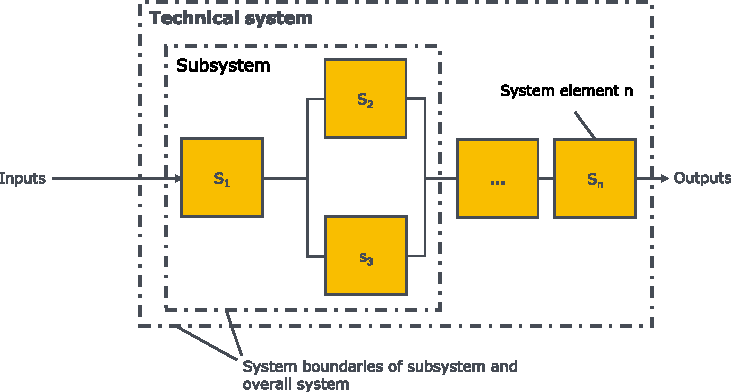
\includegraphics[width=\linewidth]{fig/lec01/tech_system.pdf}
			\caption*{System and subsystem of a technical system (source: Weyrich, M., 2024. Industrial Automation and Information Technology. Berlin, Germany: Springer.)}
		\end{figure}
	\end{column}
	\begin{column}{0.45\textwidth}
		\textbf{Key points}
		\begin{itemize}
		\item Each subsystem has a specific function (mapping of input $\rightarrow$ output).
		\item Abstraction helps describe and model complex installations independent of their concrete hardware.
		\end{itemize}
		\textbf{Reading the diagram}\\
		\footnotesize
		Inputs are processed through subsystems $S_1,\ldots,S_n$ within defined system boundaries to produce outputs. Subsystems can themselves contain elements and control logic.
	\end{column}
\end{columns}
\end{frame}


\begin{frame}{Technical Facility — Concrete Realization}
\textbf{Definition}\\
A \textbf{technical facility} is a concrete collection of equipment, devices, and machinery that work together to achieve a purpose. It is a physical implementation of one or more technical systems.

\vspace{1.5mm}
\begin{columns}
	\begin{column}{0.55\textwidth}
		\textbf{Example (process plant excerpt)}
		\begin{itemize}
		\item Raw materials A and B; valves, piping, reactor; sensors and actuators.
		\item \textbf{Control signals} command actuators; \textbf{measurement signals} report states.
		\item Output is a new substance/product C.
		\end{itemize}
	\end{column}
	\begin{column}{0.45\textwidth}
		\begin{figure}
			\centering
			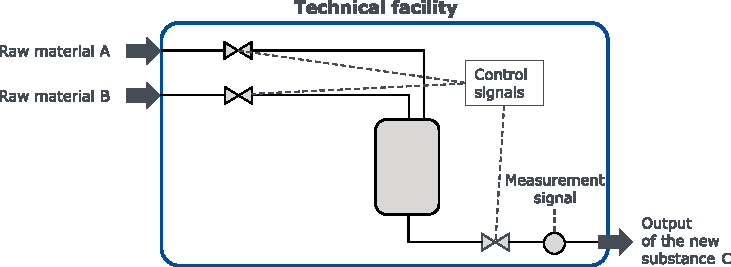
\includegraphics[width=\linewidth]{fig/lec01/tech_facility.pdf}
			\caption*{Example of a technical facility (adapted from \href{https://doi. org/10.1007/978-3-642-58446-6}{Lauber et. al.})}
		\end{figure}
	\end{column}
\end{columns}
\end{frame}

%----------------------------------------------------------
\begin{frame}{Technical Process — Functional Abstraction}
\textbf{Definition (DIN IEC 60050-351 / VDI Glossary)}\\
A \textbf{technical process} is the complete set of interacting operations by which \textbf{matter, energy, or information} is transformed, transported, or stored.

\vspace{1.5mm}
\textbf{Why abstract?}
\begin{itemize}
  \item Real-time information processing and distributed integration require a \textbf{function-oriented} view.
  \item Focus on \textbf{subprocesses}, their interrelations, and \textbf{command/state variables}.
\end{itemize}

\begin{columns}[T,onlytextwidth]
\column{0.58\textwidth}
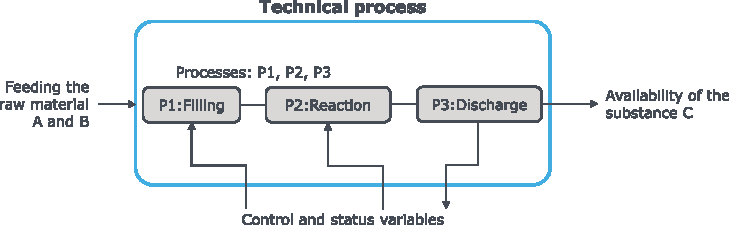
\includegraphics[width=\linewidth]{fig/lec01/example_tech_process.pdf}
\column{0.38\textwidth}
\footnotesize
\textbf{Example sequence}\\
P1: Filling \quad P2: Reaction \quad P3: Discharge\\[1mm]
Inputs: inflow A \& B \quad Output: product C\\
Measured/commanded: valve openings, flow rates, temperatures, levels.
\end{columns}
\end{frame}

%----------------------------------------------------------
\begin{frame}{Relating the Terms in Practice}
\textbf{From concrete to abstract and back}
\begin{enumerate}
  \item \textbf{Technical system} — abstract structure of subsystems and functions (what maps to what).
  \item \textbf{Technical facility} — physical realization (hardware: valves, pumps, reactors, sensors).
  \item \textbf{Technical process} — functional chain of operations (filling $\rightarrow$ reaction $\rightarrow$ discharge) with \textbf{inputs/outputs} and \textbf{state \& command variables}.
\end{enumerate}

\vspace{2mm}
\textbf{Signal viewpoints}
\begin{itemize}
  \item \emph{Inputs/Outputs}: material/energy/information entering or leaving the process.
  \item \emph{Command variables}: actuator setpoints (e.g., valve opening).
  \item \emph{State variables}: measured quantities (e.g., flow rate, temperature, level).
\end{itemize}

\vspace{2mm}
\textbf{Takeaway}\\
Use \emph{system} to reason about structure, \emph{facility} to reason about hardware, and \emph{process} to reason about operations and signals—then connect all three with software and communication to realize automation.
\end{frame}

%----------------------------------------------------------
\begin{frame}{What is an \textit{Automaton}? (DIN IEC 60050-351)}
\textbf{Definition (concise)}\\
\emph{A self-acting artificial system whose behaviour is governed by given decision rules (discretely or continuously). Its output variables are generated from its input and state variables.}

\vspace{2mm}
\textbf{Implications}
\begin{itemize}
  \item Autonomy arises from \textbf{rules/relationships} linking inputs, states, and outputs.
  \item Can operate in discrete-event fashion (sequencing) or continuous-time regulation.
  \item An \textbf{automaton} is the basic building block of automation technology.
\end{itemize}

\vspace{1mm}
\textbf{From devices to systems}
\begin{itemize}
  \item Modern automation focuses on \textbf{orchestrating subsystems} that cooperate to perform tasks.
  \item Interest shifts from isolated functions to \textbf{how functions are connected}.
\end{itemize}
\end{frame}

%----------------------------------------------------------
\begin{frame}{Automaton = Technical Process + Automation System + User}
\begin{columns}[T,onlytextwidth]
\column{0.58\textwidth}
\textbf{Constituent parts}
\begin{itemize}
  \item \textbf{Technical process}: the physical/chemical/information transformation (process step $n$ and neighbours).
  \item \textbf{Automation system}: sensors, controllers, actuators implementing the decision rules.
  \item \textbf{User (human operator)}: activates/deactivates, monitors, and intervenes in exceptions.
\end{itemize}

\textbf{Signal view}
\begin{itemize}
  \item \emph{Signals from sensors} $\rightarrow$ internal state/measurement.
  \item \emph{Signals to actuators} $\rightarrow$ commands to influence the process.
\end{itemize}

\column{0.40\textwidth}
%\centering
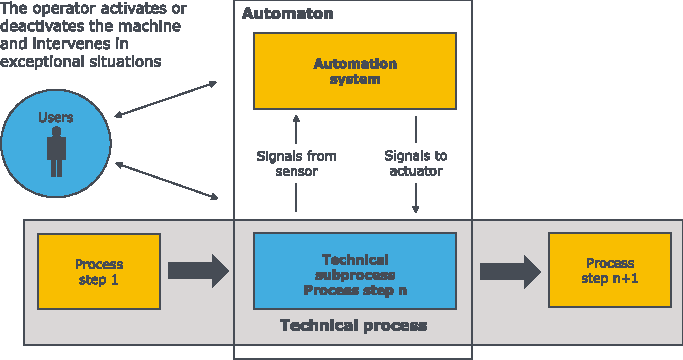
\includegraphics[width=\linewidth]{fig/lec01/automation_human_user.pdf}\\
\footnotesize{Technical system with automation and human in the loop (source: Weyrich, M., 2024. Industrial Automation and Information Technology. Berlin, Germany: Springer.)}

\textbf{Role of the human}\\
A special \textbf{monitoring} function remains; the user decides \textbf{when/where} to employ the automaton within a defined context.
\end{columns}
\end{frame}

%----------------------------------------------------------
\begin{frame}{Degree of Automation \& Taylorian Background}
\textbf{Degree of automation (DIN IEC 60050-351)}\\
\emph{Proportion of automatic functions relative to the entire set of functions of a system or facility.}

\vspace{2mm}
\textbf{Taylorism and early industrial automation}
\begin{itemize}
  \item Production decomposed into \textbf{detailed tasks} via labour studies and management.
  \item Enables direct comparison of human vs machine for \textbf{time, quality, and cost}.
  \item Example: \textbf{welding robot} executes a specified seam; quality becomes more reproducible, but setup/programming costs arise.
\end{itemize}

\vspace{1mm}
\textbf{Limits: Taylor's ``vicious circle''}
\begin{itemize}
  \item Increasingly specialized subprocesses $\Rightarrow$ complex dependencies and inflexibility.
  \item Changing functions requires significant \textbf{engineering effort}.
\end{itemize}
\end{frame}

%----------------------------------------------------------
\begin{frame}{Towards Flexible Automata}
\textbf{Raising applicability without full reprogramming}
\begin{itemize}
  \item Add \textbf{sensing} to compensate disturbances (e.g., thermal distortion during welding).
  \item Use feedback to adapt within the \textbf{dedicated function} while avoiding time-consuming reprogramming.
\end{itemize}

\vspace{2mm}
\textbf{Modern direction}
\begin{itemize}
  \item Combine \textbf{software} with \textbf{standardized \& modular systems} to increase \textbf{flexibility and applicability}.
  \item Move from isolated automata to \textbf{integrated automated systems} with coordinated functions.
\end{itemize}

\vspace{2mm}
\textbf{Design takeaway}
\begin{itemize}
  \item Specify the \emph{context of use}, the \emph{degree of automation}, and the \emph{intervention rules} for the human.
  \item Architect sensor-decision-actuation loops that allow \textbf{bounded autonomy} and graceful user override.
\end{itemize}
\end{frame}

%----------------------------------------------------------
\begin{frame}{Summary for Practice}
\begin{itemize}
  \item An \textbf{automaton} = automation system + technical process, supervised by a \textbf{user}.
  \item \textbf{Degree of automation} quantifies how much is automatic; it varies by task and context.
  \item Historical Taylorism enabled productivity but also rigidity; modern systems target \textbf{flexibility} through sensing, software, and modularity.
  \item Effective automation design balances \textbf{autonomy} with \textbf{human oversight} and clear exception handling.
\end{itemize}
\end{frame}

% % --- Slide 3: The Automation Stack (Mechatronics Lens) ---
% \begin{frame}{The Automation Stack (Mechatronics Lens)}
% \begin{columns}[T,onlytextwidth]
% \column{0.54\textwidth}
% \textbf{Layers}
% \begin{enumerate}
%   \item \textbf{Sensors} (electrical, mechanical, magnetic, optical) $\rightarrow$ scaling, filtering, calibration, shielding.
%   \item \textbf{Compute} (MCU/DSP, FPGA, PLC): timing, determinism, safety tasks, OS/RTOS.
%   \item \textbf{Control \& Sequencing}: PID/IMC, cascades, feedforward; SFC/state machines, interlocks, mode logic.
%   \item \textbf{Actuators \& Drives}: DC/BLDC/servo, VFD/FOC, motion profiles, STO.
%   \item \textbf{Comms \& Data}: OPC~UA, Modbus‐TCP, MQTT; time sync, historians, dashboards.
%   \item \textbf{Supervision \& Optimization}: HMI/SCADA, digital twins, KPIs (OEE), diagnostics, updates.
% \end{enumerate}

% \column{0.44\textwidth}
% \centering
% %\includegraphics[width=\linewidth]{stack_placeholder.png}\\[-1mm]
% \footnotesize{Block diagram placeholder: Sensor $\to$ Conditioning $\to$ Compute $\to$ Actuator, with data to SCADA/Cloud.}
% \end{columns}

% \vspace{1mm}
% \textbf{System integrator view} \\
% Automation engineers orchestrate multiple “couples” (machines/cells) to dance in unison: coordination, timing, safety, and lifecycle management.
% \end{frame}


%%%%%%%%%%%%%%%%%%%%%%%%%%%%%%%%%%%%%%%%%%%%%%%%%%%%%%%%%%%%%
%% Necessary prior knowledge %%
%%%%%%%%%%%%%%%%%%%%%%%%%%%%%%%%%%%%%%%%%%%%%%%%%%%%%%%%%%%%%
\begin{frame}
	\frametitle{Necessary prior knowledge for this course}
	You should have a basic understanding of the following topics:
	\begin{itemize}
		\item Basic electrical engineering knowledge (e.g., Ohm's law, Kirchhoff's laws, etc.)
		\item Basic understanding of physics in electronics
		\item Algebra and complex numbers
		\item Basic signal theory knowledge (e.g., Fourier series, Laplace transform)
		\item No advanced knowledge of semiconductors or programming is needed — this course builds those concepts from scratch and applies them to real systems.
	\end{itemize}
	\vspace{0.5cm}
	\onslide<2->What we will \underline{not} cover, but you do not need to know (covered in separate courses):
	\begin{itemize}
		\item Power converter circuits and topologies.
		\item Power electronics in depth involving analysis and controller design. 
	\end{itemize}
\end{frame}

%%%%%%%%%%%%%%%%%%%%%%%%%%%%%%%%%%%%%%%%%%%%%%%%%%%%%%%%%%%%%
%% Recommended reading %%
%%%%%%%%%%%%%%%%%%%%%%%%%%%%%%%%%%%%%%%%%%%%%%%%%%%%%%%%%%%%%
\begin{frame}
	\frametitle{Recommended reading}
	\begin{itemize}
		\item Baliga, B. Jayant. Fundamentals of power semiconductor devices. Springer Science \& Business Media, 2010.
		\item Lutz, Josef, Heinrich Schlangenotto, Uwe Scheuermann, and Rik De Doncker. "Semiconductor power devices." Physics, characteristics, reliability 2 (2011).
		\item Baliga, B. Jayant, ed. Wide Bandgap Semiconductor Power Devices: Materials, Physics, Design, and Applications. Woodhead Publishing, 2018.
		\item K. Niayesh, M. Runde, "Power Switching Components Theory, Applications and Future Trends", 1. Ed., Springer, 2018.
	\end{itemize}
\end{frame}